\documentclass[10pt]{article}
\usepackage[utf8]{inputenc}
\usepackage[T1]{fontenc}
\usepackage{amsmath}
\usepackage{amsfonts}
\usepackage{amssymb}
\usepackage[version=4]{mhchem}
\usepackage{stmaryrd}
\usepackage{bbold}
\usepackage{graphicx}
\usepackage[export]{adjustbox}
\graphicspath{ {./images/} }
\usepackage{mathrsfs}

\title{Kernel Ridge Regression and the Kernel Trick }

\author{}
\date{}


\begin{document}
\maketitle
Machine Learning Course - CS-433

Oct 31, 2023

Nicolas Flammarion

EPFL

\section*{Equivalent formulations for ridge regression}
Objective

$$
\min _{w} \frac{1}{2 N} \sum_{n=1}^{N}\left(y_{n}-w^{\top} x_{n}\right)^{2}+\frac{\lambda}{2}\|w\|^{2}
$$

The solution is given by

$$
\begin{aligned}
& \mathcal{W}_{*}=\frac{1}{N}\left(\frac{1}{N} \mathbf{X}^{\top} \mathbf{X}+\lambda I_{d}\right)^{-1} \mathbf{X}^{\top} \mathbf{y} \\
& \mathbf{X}^{\top} \in \mathbb{R}^{d \times N} \rightarrow d \times d
\end{aligned}
$$

Alternatively, the solution can be written as

$$
\mathcal{W}_{*}=\frac{1}{N} \mathbf{X}^{\top}(\underbrace{\frac{1}{N} \mathbf{X X}^{\top}+\lambda I_{N}}_{\mathbf{X} \in \mathbb{R}^{N \times d}})^{-1} \mathbf{y}
$$

Proof: Let $P \in \mathbb{R}^{m \times n}$ and $Q \in \mathbb{R}^{n \times m}$

$$
P\left(Q P+I_{n}\right)=P Q P+P=\left(P Q+I_{m}\right) P
$$

Assuming that both $Q P+I_{n}$ and $P Q+I_{m}$ are invertible

$$
\left(P Q+I_{m}\right)^{-1} P=P\left(Q P+I_{n}\right)^{-1}
$$

We deduce the result with $P=\mathbf{X}^{\top}$ and $Q=\frac{1}{\lambda N} \mathbf{X}$

$$
\begin{aligned}
\mathcal{W}_{*} & =\frac{1}{N}(\underbrace{\left.\frac{1}{N} \mathbf{X}^{\top} \mathbf{X}+\lambda I_{d}\right)^{-1} \mathbf{X}^{\top} \mathbf{y}}_{\rightarrow d \times d} \\
\mathbf{X}^{\top} & \in \mathbb{R}^{d \times N} \rightarrow d{ }^{-1}
\end{aligned}
$$

But it can be alternatively written as

$$
\mathcal{W}_{*}=\frac{1}{N} \mathbf{X}^{\top}(\underbrace{\frac{1}{N} \mathbf{X X}^{\top}+\lambda I_{N}}_{\mathbf{X} \in \mathbb{R}^{N \times d}})^{-1} \mathbf{y}
$$

\section*{Usefulness of the alternative form}
$$
\mathcal{W}_{*}=\underbrace{\frac{1}{N} \mathbf{X}^{\top}}_{d \times N}(\underbrace{\frac{1}{N} \mathbf{X X}^{\top}+\lambda I_{N}}_{N \times N})^{-1} \mathbf{y}
$$

\begin{enumerate}
  \item Computational complexity:
\end{enumerate}

\begin{itemize}
  \item For the original formulation $\frac{1}{N}\left(\frac{1}{N} \mathbf{X}^{\top} \mathbf{X}+\lambda I_{d}\right)^{-1} \mathbf{X}^{\top} \mathbf{y}, O\left(d^{3}+N d^{2}\right)$
  \item For the new formulation $\frac{1}{N} \mathbf{X}^{\top}\left(\frac{1}{N} \mathbf{X} \mathbf{X}^{\top}+\lambda I_{N}\right)^{-1} \mathbf{y}, O\left(N^{3}+d N^{2}\right)$
\end{itemize}

$\Rightarrow$ Depending on $d, N$ one formulation may be more efficient than the other

\begin{enumerate}
  \setcounter{enumi}{1}
  \item Structural difference:
\end{enumerate}

$$
w_{*}=\mathbf{X}^{\top} \alpha_{*} \text { where } \alpha_{*}=\frac{1}{N}\left(\frac{1}{N} \mathbf{X} \mathbf{X}^{\top}+\lambda I_{N}\right)^{-1} \mathbf{y}
$$

$\Rightarrow w_{*} \in \operatorname{span}\left\{x_{1}, \cdots, x_{N}\right\}$

These two insights are fundamental to understanding the kernel trick

\section*{Representer Theorem}
Claim: For any loss function $\ell$, there exists $\alpha_{*} \in \mathbb{R}^{N}$ such that

$$
w_{*}:=\mathbf{X}^{\top} \alpha_{*} \in \arg \min _{w} \frac{1}{N} \sum_{n=1}^{N} \ell\left(x_{n}^{\top} w, y_{n}\right)+\frac{\lambda}{2}\|w\|^{2}
$$

Meaning: There exists an optimal solution within $\operatorname{span}\left\{x_{1}, \cdots, x_{N}\right\}$

Consequence: This is more general than LS, enabling the kernel trick to various problems, including Kernel SVM, Kernel LS, and Kernel Principal Component Analysis

\section*{Proof of the representer theorem}
Let $w_{*}$ be an optimal solution of $\min _{w} \frac{1}{N} \sum_{n=1}^{N} \ell\left(x_{n}^{\top} w, y_{n}\right)+\frac{\lambda}{2}\|w\|^{2}$

We can always rewrite $w_{*}$ as $w_{*}=\sum_{n=1}^{N} \alpha_{n} x_{n}+u$ where $u^{\top} x_{n}=0$ for all $n$

Let's define $w=w_{*}-u$

\begin{itemize}
  \item $\left\|w_{*}\right\|^{2}=\|w\|^{2}+\|u\|^{2}$, thus $\|w\|^{2} \leq\left\|w_{*}\right\|^{2}$

  \item For all $n, w^{\top} x_{n}=\left(w_{*}-u\right)^{\top} x_{n}=w_{*}^{\top} x_{n}$, thus $\ell\left(x_{n}^{\top} w, y_{n}\right)=\ell\left(x_{n}^{\top} w_{*}, y_{n}\right)$

\end{itemize}

Therefore

$$
\frac{1}{N} \sum_{n=1}^{N} \ell\left(x_{n}^{\top} w, y_{n}\right)+\frac{\lambda}{2}\|w\|^{2} \leq \frac{1}{N} \sum_{n=1}^{N} \ell\left(x_{n}^{\top} w_{*}, y_{n}\right)+\frac{\lambda}{2}\left\|w_{*}\right\|^{2}
$$

And $w$ is an optimal solution for this problem.

\section*{Kernelized ridge regression}
Classic formulation in $w$ :

$$
w_{*}=\arg \min _{w} \frac{1}{2 N}\|\mathbf{y}-\mathbf{X} w\|^{2}+\frac{\lambda}{2}\|w\|^{2}
$$

Alternative formulation in $\alpha$ :

$$
\alpha_{*}=\arg \min _{\alpha} \frac{1}{2} \alpha^{\top}\left(\frac{1}{N} \mathbf{X} \mathbf{X}^{\top}+\lambda I_{N}\right) \alpha-\frac{1}{N} \alpha^{\top} \mathbf{y}
$$

Claim: These two formulations are equivalent

Proof: Set the gradient to 0 , to obtain $\alpha_{*}=\frac{1}{N}\left(\frac{1}{N} \mathbf{X} \mathbf{X}^{\top}+\lambda I_{N}\right)^{-1} \mathbf{y}$, and $w_{*}=\mathbf{X}^{\top} \alpha_{*}$

Key takeaways:

\begin{itemize}
  \item Computational complexity - depending on $d, N$
  \item The dual formulation only uses $\mathbf{X}$ through the kernel matrix $\mathbf{K}=\mathbf{X X}^{\top}$
\end{itemize}

\section*{Kernel matrix}
$$
\mathbf{K}=\mathbf{X} \mathbf{X}^{\top}=\left(\begin{array}{cccc}
x_{1}^{\top} x_{1} & x_{1}^{\top} x_{2} & \cdots & x_{1}^{\top} x_{N} \\
x_{2}^{\top} x_{1} & x_{2}^{\top} x_{2} & \cdots & x_{2}^{\top} x_{N} \\
\vdots & \vdots & \ddots & \vdots \\
x_{N}^{\top} x_{1} & x_{N}^{\top} x_{2} & \cdots & x_{N}^{\top} x_{N}
\end{array}\right)=\left(x_{i}^{\top} x_{j}\right)_{i, j} \in \mathbb{R}^{N \times N}
$$

\section*{Embedding into feature spaces}
\begin{center}
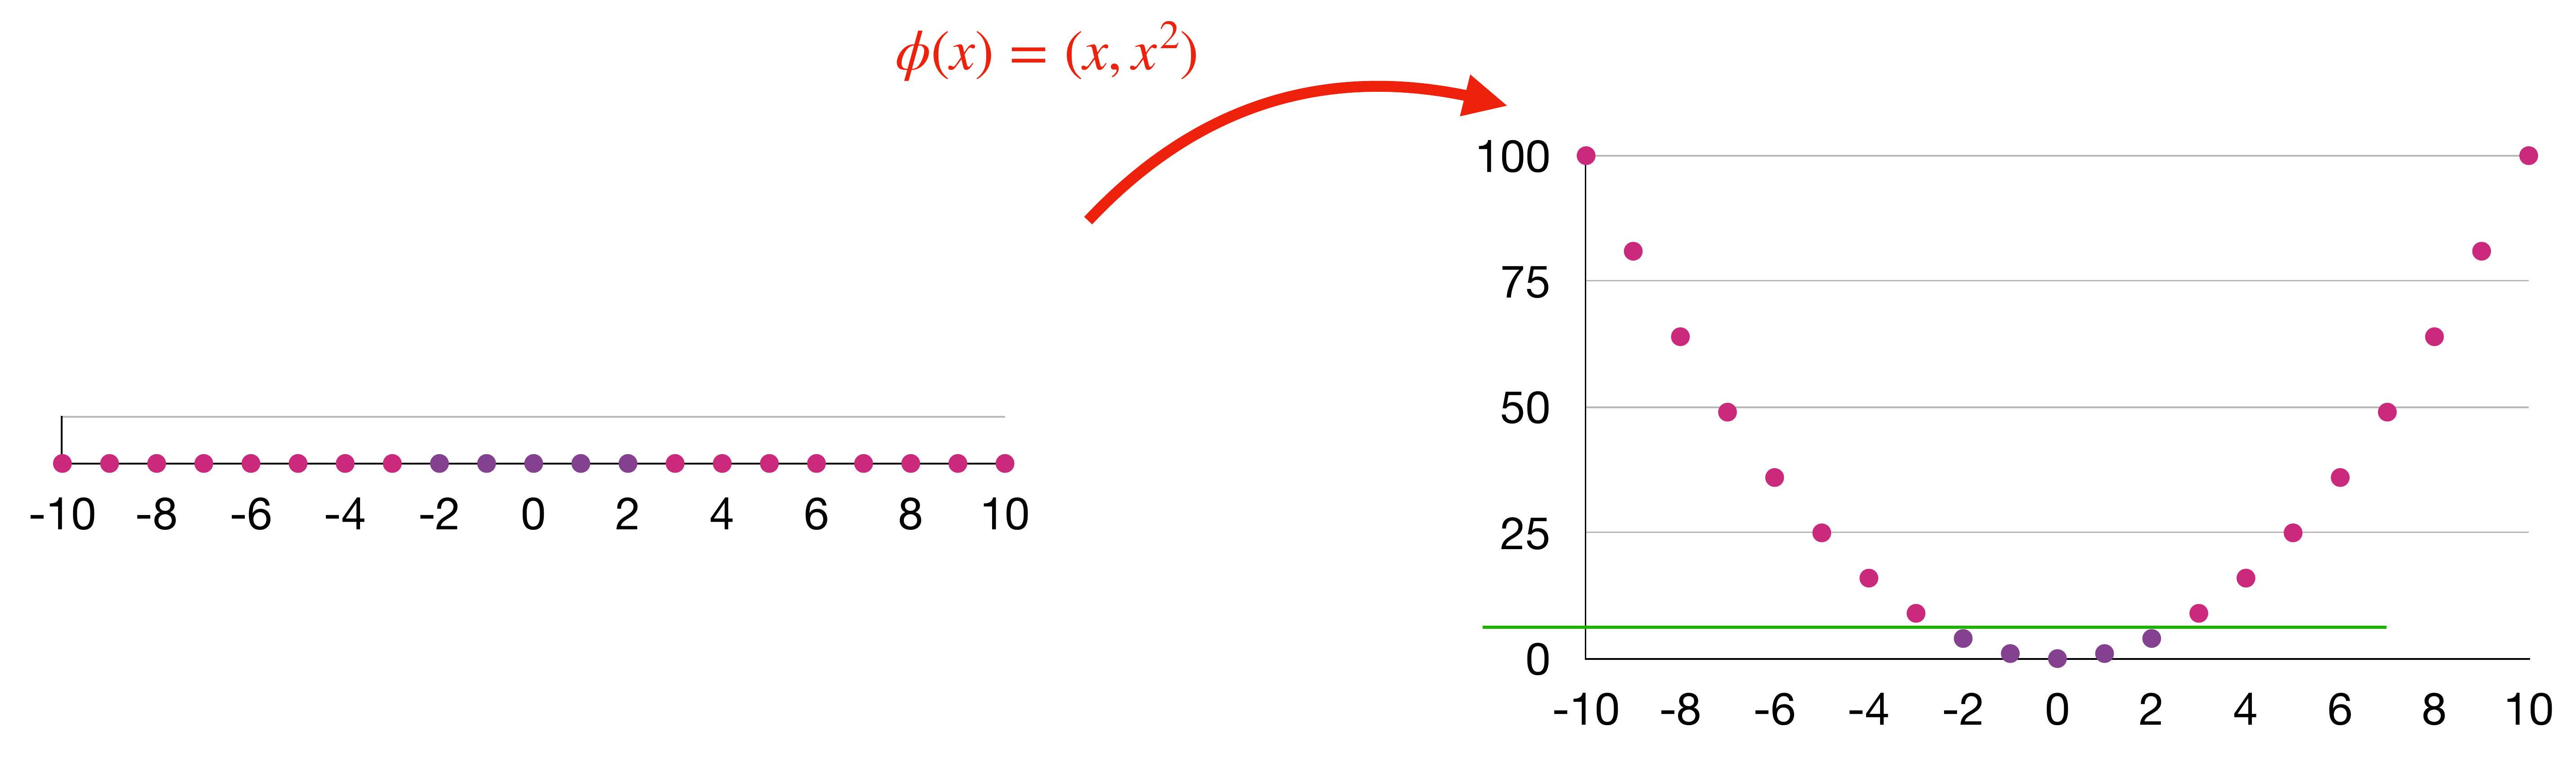
\includegraphics[max width=\textwidth]{2023_12_30_94b0d65233167cf65e4cg-09}
\end{center}

\section*{Usefulness of feature spaces}
\begin{center}
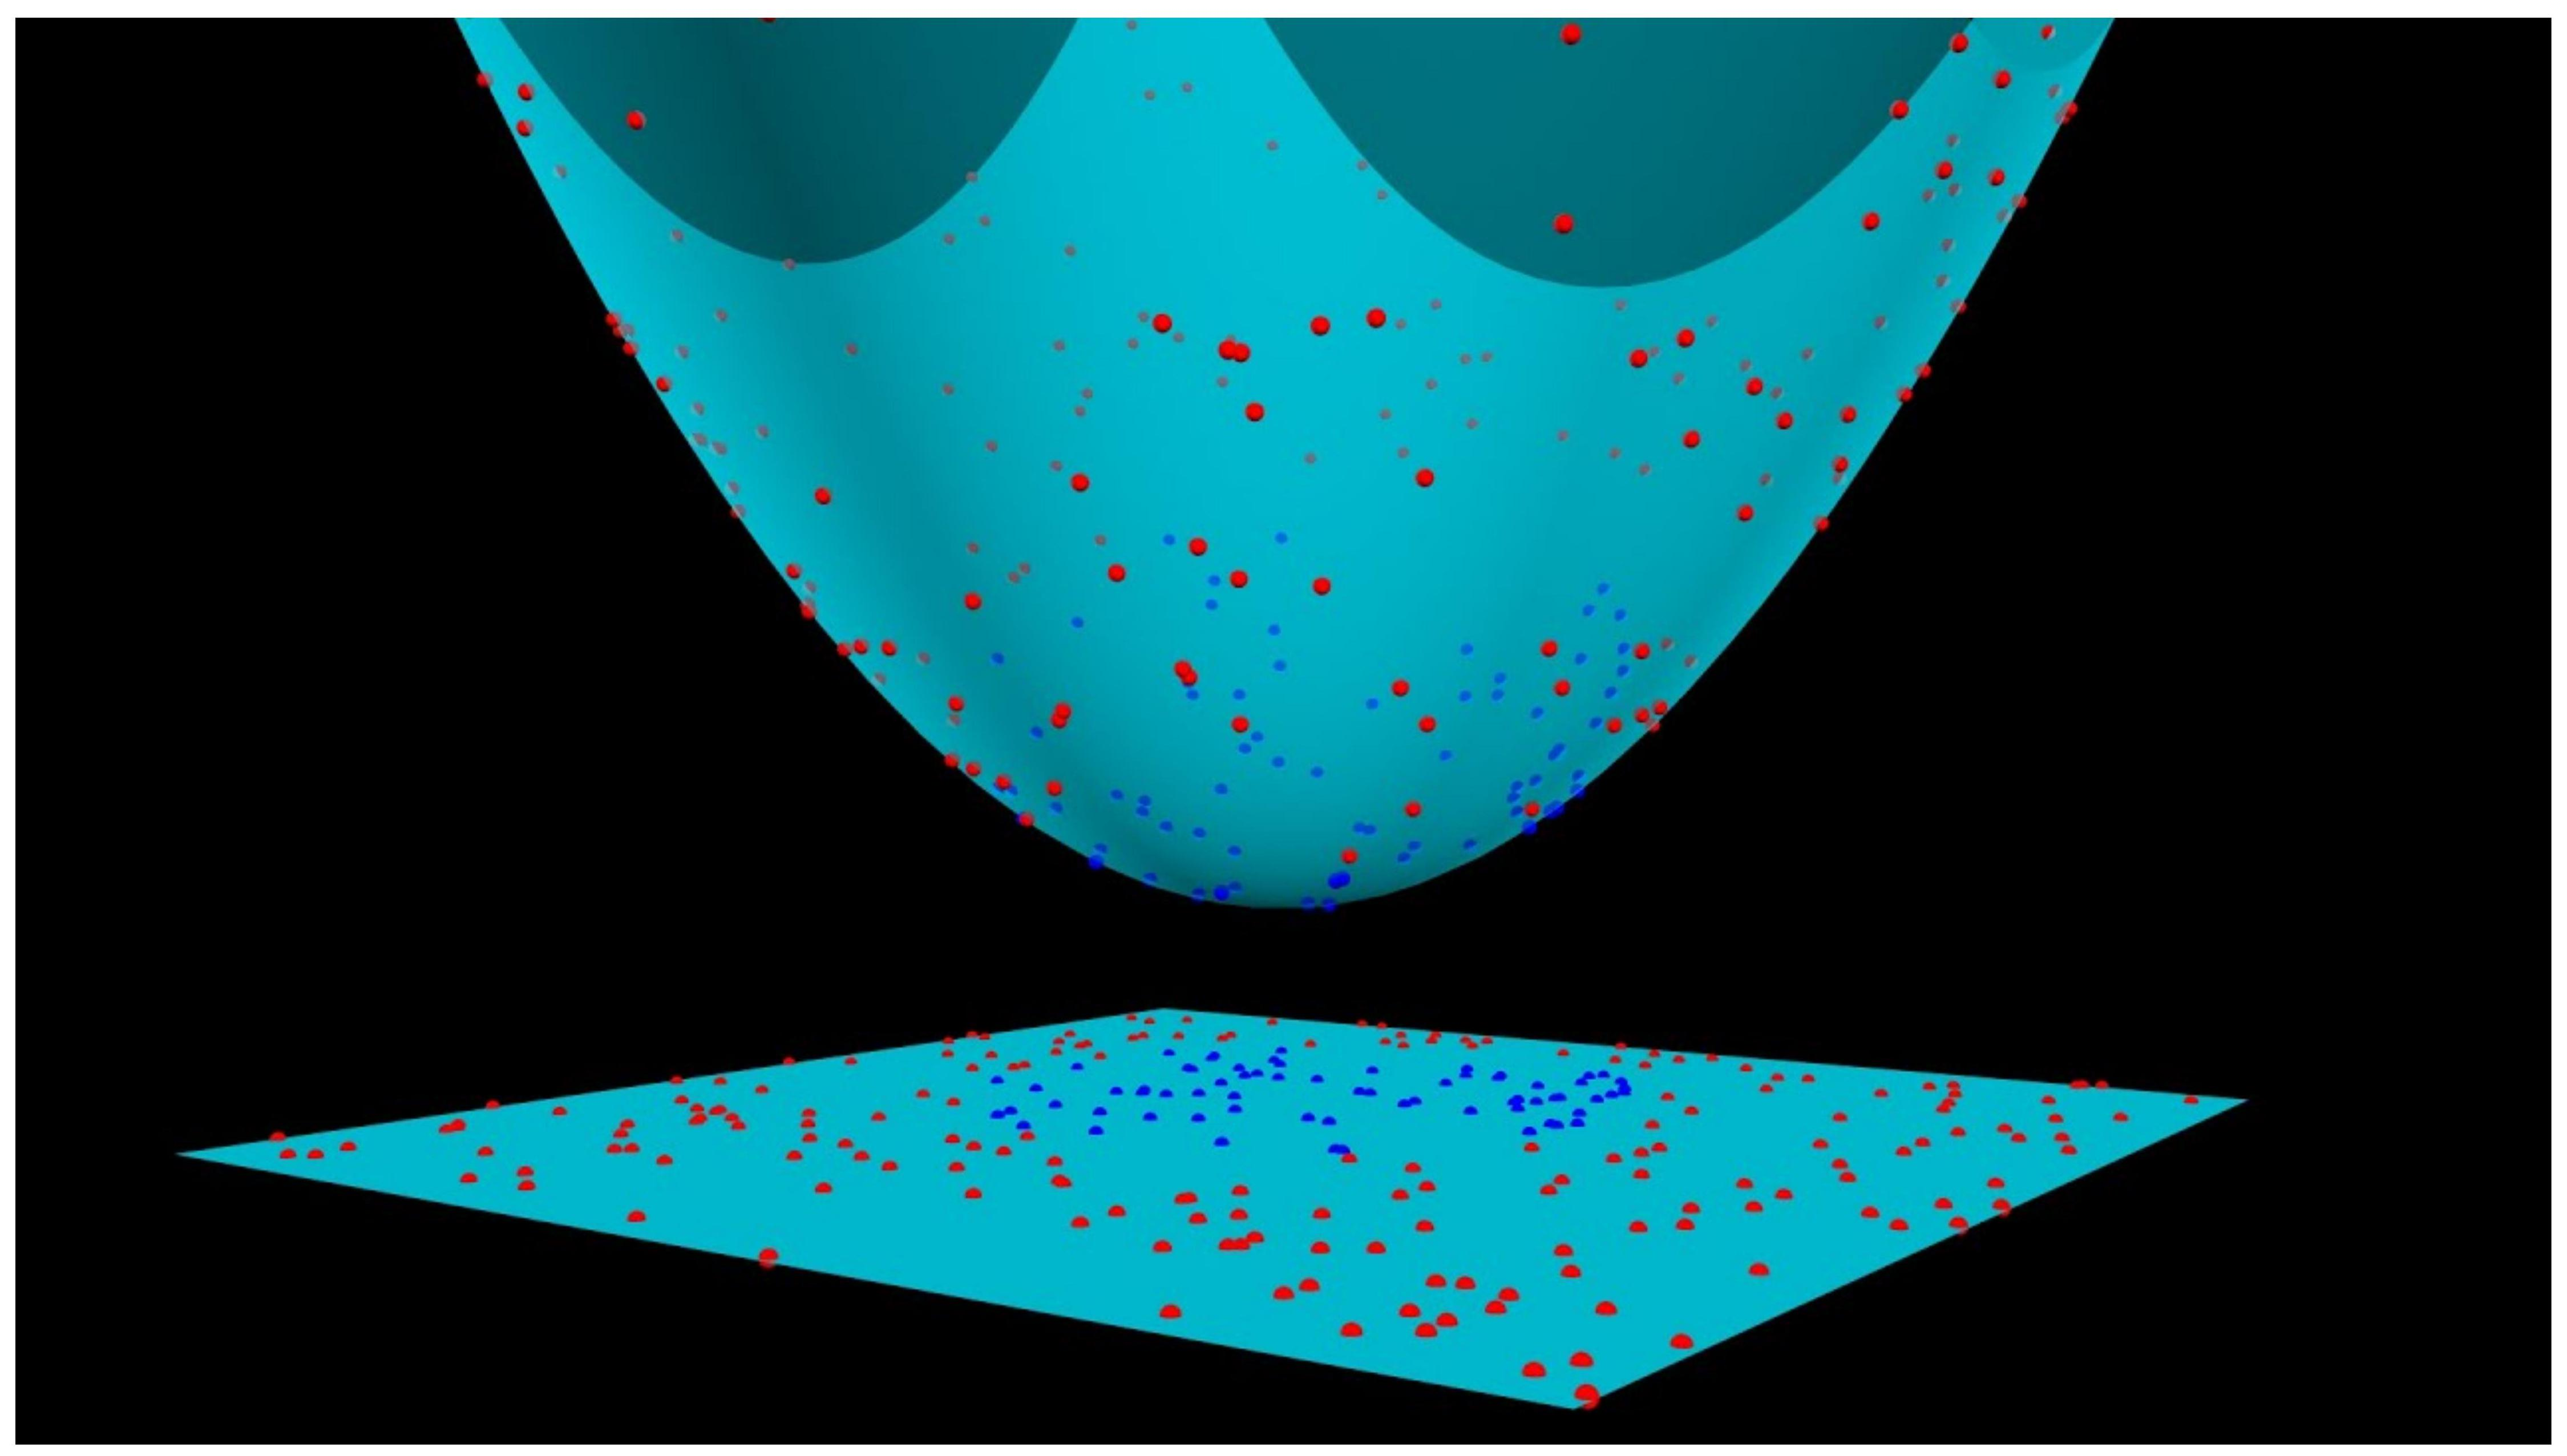
\includegraphics[max width=\textwidth]{2023_12_30_94b0d65233167cf65e4cg-10}
\end{center}

\section*{Kernel matrix with feature spaces}
When a feature map $\phi: \mathbb{R}^{d} \rightarrow \mathbb{R}^{\tilde{d}}$ is used,

$$
\left(x_{n}\right)_{n=1}^{N} \hookrightarrow\left(\phi\left(x_{n}\right)\right)_{n=1}^{N}
$$

The associated kernel matrix is

$$
\mathbf{K}=\boldsymbol{\Phi} \boldsymbol{\Phi}^{\top}=\left(\begin{array}{cccc}
\phi\left(x_{1}\right)^{\top} \phi\left(x_{1}\right) & \phi\left(x_{1}\right)^{\top} \phi\left(x_{2}\right) & \cdots & \phi\left(x_{1}\right)^{\top} \phi\left(x_{N}\right) \\
\phi\left(x_{2}\right)^{\top} \phi\left(x_{1}\right) & \phi\left(x_{2}\right)^{\top} \phi\left(x_{2}\right) & \cdots & \phi\left(x_{2}\right)^{\top} \phi\left(x_{N}\right) \\
\vdots & \vdots & \ddots & \vdots \\
\phi\left(x_{N}\right)^{\top} \phi\left(x_{1}\right) & \phi\left(x_{N}\right)^{\top} \phi\left(x_{2}\right) & \cdots & \phi\left(x_{N}\right)^{\top} \phi\left(x_{N}\right)
\end{array}\right) \in \mathbb{R}^{N \times N}
$$

Problem: when $d \lll \tilde{d}$ computing $\phi(x)^{\top} \phi\left(x^{\prime}\right)$ costs $O(\tilde{d})$ - too expensive

\section*{Kernel trick}
Kernel function: $\kappa\left(x, x^{\prime}\right)$ such that

\begin{center}
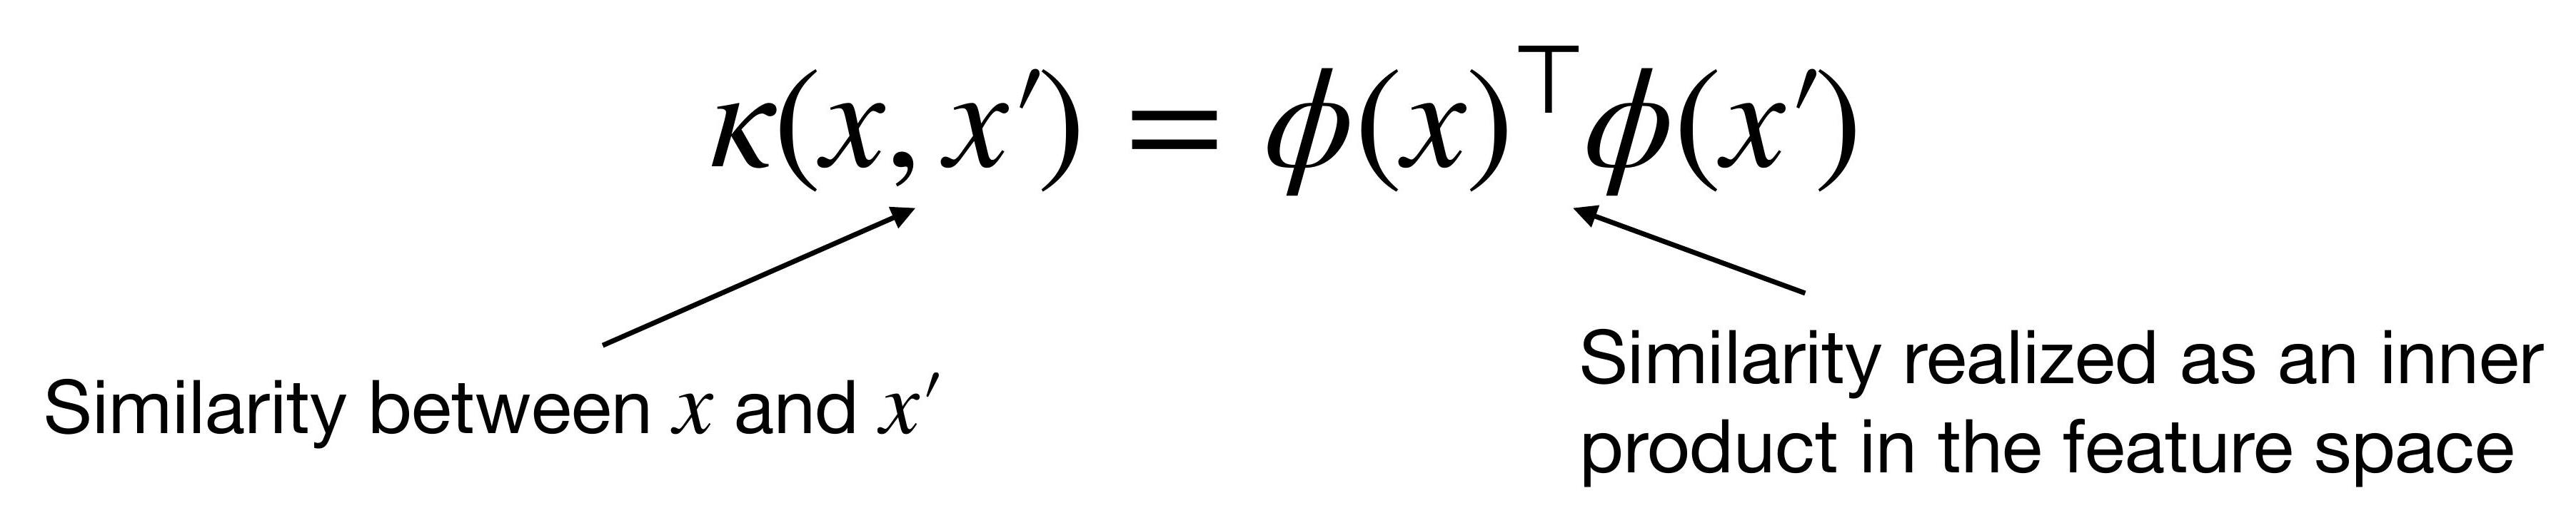
\includegraphics[max width=\textwidth]{2023_12_30_94b0d65233167cf65e4cg-12}
\end{center}

It is equivalent to

\begin{itemize}
  \item Directly compute $\kappa\left(x, x^{\prime}\right)$
  \item First map the features to $\phi(x)$, then compute $\phi(x)^{\top} \phi\left(x^{\prime}\right)$
\end{itemize}

Purpose: enable computation of linear classifiers in high-dimensional space without performing computations in this high-dimensional space directly.

\section*{Predicting with kernels}
Problem: The prediction is $y=\phi(x)^{\top} w_{*}$ but computing $\phi(x)$ can be expensive

Question: How can we make predictions using only the kernel function, without the need to compute $\phi(x)$ ?

Answer: $\quad \phi(x)^{\top} w_{*}=\phi(x)^{\top} \phi(\mathbf{X})^{\top} \alpha_{*}=\sum_{n=1}^{N} \kappa\left(x, x_{n}\right) \alpha_{*_{n}}$ We can do a prediction only using the kernel function

Important remark:

$$
\underline{y=\phi(x)^{\top} w_{*}=f_{W_{*}}(x)}
$$

Linear prediction

in the feature space
Non linear prediction

in the $\mathscr{X}$ space

\section*{Examples of kernel (easy)}
\begin{enumerate}
  \item Linear kernel: $\kappa\left(x, x^{\prime}\right)=x^{\top} x^{\prime}$
\end{enumerate}

$\rightarrow$ Feature map is $\phi(x)=x$

\begin{enumerate}
  \setcounter{enumi}{1}
  \item Quadratic kernel: $\kappa\left(x, x^{\prime}\right)=\left(x x^{\prime}\right)^{2}$ for $x, x^{\prime} \in \mathbb{R}$
\end{enumerate}

$\Rightarrow$ Feature map is $\phi(x)=x^{2}$

\section*{3. Polynomial kernel}
Let $x, x^{\prime} \in \mathbb{R}^{3}$

$$
\kappa\left(x, x^{\prime}\right)=\left(x_{1} x_{1}^{\prime}+x_{2} x_{2}^{\prime}+x_{3} x_{3}^{\prime}\right)^{2}
$$

Feature map:

Proof:

$$
\phi(x)=\left[x_{1}^{2}, x_{2}^{2}, x_{3}^{2}, \sqrt{2} x_{1} x_{2}, \sqrt{2} x_{1} x_{3}, \sqrt{2} x_{2} x_{3}\right] \in \mathbb{R}^{6}
$$

$$
\begin{aligned}
\kappa\left(x, x^{\prime}\right) & =\phi(x)^{\top} \phi\left(x^{\prime}\right) \\
\kappa\left(x, x^{\prime}\right) & =\left(x_{1} x_{1}^{\prime}+x_{2} x_{2}^{\prime}+x_{3} x_{3}^{\prime}\right)^{2} \\
& =\left(x_{1} x_{1}^{\prime}\right)^{2}+\left(x_{2} x_{2}^{\prime}\right)^{2}+\left(x_{3} x_{3}^{\prime}\right)^{2}+2 x_{1} x_{2} x_{1}^{\prime} x_{2}^{\prime}+2 x_{1} x_{3} x_{1}^{\prime} x_{3}^{\prime}+2 x_{2} x_{3} x_{2}^{\prime} x_{3}^{\prime} \\
& =\left(x_{1}^{2}, x_{2}^{2}, x_{3}^{2}, \sqrt{2} x_{1} x_{2}, \sqrt{2} x_{1} x_{3}, \sqrt{2} x_{2} x_{3}\right)^{\top}\left(x_{1}^{\prime 2}, x_{2}^{\prime 2}, x_{3}^{\prime 2}, \sqrt{2} x_{1}^{\prime} x_{2}^{\prime}, \sqrt{2} x_{1}^{\prime} x_{3}^{\prime}, \sqrt{2} x_{2}^{\prime} x_{3}^{\prime}\right)
\end{aligned}
$$

We obtain $\phi$ by identification

\section*{4. Radial basis function (RBF) kernel}
Let $x, x^{\prime} \in \mathbb{R}^{d}$

$$
\kappa\left(x, x^{\prime}\right)=e^{-\left(x-x^{\prime}\right)^{\top}\left(x-x^{\prime}\right)}
$$

For $x, x^{\prime} \in \mathbb{R}$

$$
\kappa\left(x, x^{\prime}\right)=e^{-\left(x-x^{\prime}\right)^{2}}
$$

Feature map:

$$
\phi(x)=e^{-x^{2}}\left(\cdots, \frac{2^{k / 2} x^{k}}{\sqrt{k !}} \cdots\right)
$$

Proof: $\quad \kappa\left(x, x^{\prime}\right)=e^{-x^{2}-x^{2}+2 x x^{\prime}}$

$$
=e^{-x^{2}} e^{-x^{\prime 2}} \sum_{k=0}^{\infty} \frac{2^{k} x^{k} x^{\prime k}}{k !} \text { by the Taylor expansion of } \exp
$$

$$
\phi(x)=e^{-x^{2}}\left(\cdots, \frac{2^{k / 2} x^{k}}{\sqrt{k !}} \cdots\right) \Longrightarrow \phi(x)^{\top} \phi\left(x^{\prime}\right)=\kappa\left(x, x^{\prime}\right)
$$

Interest: it cannot be represented as an inner product in a finite-dimensional space

\section*{Building new kernels from existing kernels}
Let $\kappa_{1}, \kappa_{2}$ be two kernel functions and $\phi_{1}, \phi_{2}$ the corresponding feature maps

Claim 1: Positive linear combinations of kernel are kernels

$$
\kappa\left(x, x^{\prime}\right)=\alpha \kappa_{1}\left(x, x^{\prime}\right)+\beta \kappa_{2}\left(x, x^{\prime}\right) \text { for } \alpha, \beta \geq 0
$$

Claim 2: Products of kernels are kernels

$$
\kappa\left(x, x^{\prime}\right)=\kappa_{1}\left(x, x^{\prime}\right) \kappa_{2}\left(x, x^{\prime}\right)
$$

Objective: To provide building blocks for deriving new kernels

Proof 1:

$$
\begin{aligned}
& \kappa\left(x, x^{\prime}\right)=\alpha \kappa_{1}\left(x, x^{\prime}\right)+\beta \kappa_{2}\left(x, x^{\prime}\right) \\
& =\alpha \phi_{1}(x)^{\top} \phi_{1}\left(x^{\prime}\right)+\beta \phi_{2}(x)^{\top} \phi_{2}\left(x^{\prime}\right) \\
& =\phi(x)^{\top} \phi\left(x^{\prime}\right) \\
& \text { where } \phi(x)=\left(\begin{array}{c}
\sqrt{\alpha} \phi_{1}(x) \\
\sqrt{\beta} \phi_{2}(x)
\end{array}\right) \in \mathbb{R}^{d_{1}+d_{2}}
\end{aligned}
$$

\section*{kernels from old kernel}
s and $\phi_{1}, \phi_{2}$ the corresponding feature maps

Claim 1: Positive linear combinations of kernel are kernel

$$
\kappa\left(x, x^{\prime}\right)=\alpha \kappa_{1}\left(x, x^{\prime}\right)+\beta \kappa_{2}\left(x, x^{\prime}\right)
$$

Claim 2: Products of kernels are kernel

$$
\kappa\left(x, x^{\prime}\right)=\kappa_{1}\left(x, x^{\prime}\right) \kappa_{2}\left(x, x^{\prime}\right)
$$

Proof 2:

$\kappa\left(x, x^{\prime}\right)=\kappa_{1}\left(x, x^{\prime}\right) \kappa_{2}\left(x, x^{\prime}\right)$

$$
=\phi_{1}(x)^{\top} \phi_{1}\left(x^{\prime}\right) \phi_{2}(x)^{\top} \phi_{2}\left(x^{\prime}\right)
$$

Let

$\phi(x)^{\top}=\left(\left(\phi_{1}(x)\right)_{1}\left(\phi_{2}(x)\right)_{1}, \cdots,\left(\phi_{1}(x)\right)_{1}\left(\phi_{2}(x)\right)_{d_{2}}, \cdots,\left(\phi_{1}(x)\right)_{d_{1}}\left(\phi_{2}(x)\right)_{1}, \cdots,\left(\phi_{1}(x)\right)_{d_{1}}\left(\phi_{2}(x)\right)_{d_{2}}\right) \in \mathbb{R}^{d_{1} d_{2}}$ then

$$
\begin{aligned}
\phi(x)^{\top} \phi\left(x^{\prime}\right) & =\sum_{i, j}\left(\phi_{1}(x)\right)_{i}\left(\phi_{2}(x)\right)_{j}\left(\phi_{1}\left(x^{\prime}\right)\right)_{i}\left(\phi_{2}\left(x^{\prime}\right)\right)_{j} \\
& =\sum_{i}\left(\phi_{1}(x)\right)_{i}\left(\phi_{1}\left(x^{\prime}\right)\right)_{i} \sum_{j}\left(\phi_{2}(x)\right)_{j}\left(\phi_{2}\left(x^{\prime}\right)\right)_{j} \\
& =\phi_{1}(x)^{\top} \phi_{1}\left(x^{\prime}\right) \phi_{2}(x)^{\top} \phi_{2}\left(x^{\prime}\right)=\kappa\left(x, x^{\prime}\right)
\end{aligned}
$$

Claim 2: Products of kernels are kernel

$$
\kappa\left(x, x^{\prime}\right)=\kappa_{1}\left(x, x^{\prime}\right) \kappa_{2}\left(x, x^{\prime}\right)
$$

\section*{Mercer's condition}
Question: Given a kernel function $\kappa$, how can we ensure the existence of a feature map $\phi$ such that

$$
\kappa\left(x, x^{\prime}\right)=\phi(x)^{\top} \phi\left(x^{\prime}\right)
$$

Answer: It is true if and only if the following Mercer's conditions are fulfilled:

\begin{itemize}
  \item The kernel function is symmetric:
\end{itemize}

$$
\forall x, x^{\prime}, \kappa\left(x, x^{\prime}\right)=\kappa\left(x^{\prime}, x\right)
$$

\begin{itemize}
  \item The kernel matrix is psd for all possible input sets:
\end{itemize}

$$
\forall N \geq 0, \forall\left(x_{n}\right)_{n=1}^{N}, \quad \mathbf{K}=\left(\kappa\left(x_{i}, x_{j}\right)\right)_{i, j=1}^{N} \geqslant 0
$$

\section*{Recap}
\begin{itemize}
  \item Many algorithms (SVM, Least Squares, PCA, etc) can be rewritten so that they rely only on inner products between data points $\left(\mathbf{X X}^{\top}\right)$

  \item This motivates to generalize the inner products with kernels to make the model non-linear in the input space

  \item This can improve efficiency by avoiding a direct computation of feature maps $\phi(x)$ of a potentially high-dimensional space

  \item To predict with kernels, you need to compute the similarity $k\left(x, x_{i}\right)$ of a new point $x$ with every training point $x_{i}$

  \item You can derive new kernels using a certain set of properties

\end{itemize}

\section*{Bonus: proof of Mercer theorem}
\begin{itemize}
  \item If $\kappa$ represents an inner product then it is symmetric and the kernel matrix is psd:
\end{itemize}

$$
v^{\top} \mathrm{K} v=\sum_{i, j} v_{i} v_{j} \phi\left(x_{i}\right)^{\top} \phi\left(x_{j}\right)=\left\|\sum_{i} v_{i} \phi\left(x_{i}\right)\right\|^{2}
$$

\begin{itemize}
  \item Define $\phi(x)=\kappa(\cdot, x)$. Define a vector space of functions by considering all linear combinations $\left\{\sum_{i} \alpha_{i} \kappa\left(\cdot, x_{i}\right)\right\}$. Define an inner product on this vector space by
\end{itemize}

$$
\left\langle\sum_{i} \alpha_{i} \kappa\left(\cdot, x_{i}\right), \sum_{j} \beta_{j} \kappa\left(\cdot, x_{j}^{\prime}\right)\right\rangle=\sum_{i, j} \alpha_{i} \beta_{j} \kappa\left(x_{i}, x_{j}^{\prime}\right)
$$

This is a valid inner product (symmetric, bilinear and positive definite, with equality holding only if $\phi(x)$ is the zero function)

Consequently

$$
\left\langle\phi(x), \phi\left(x^{\prime}\right)\right\rangle=\left\langle\kappa(\cdot, x), \kappa\left(\cdot, x^{\prime}\right)\right\rangle=\kappa\left(x, x^{\prime}\right)
$$


\end{document}